\documentclass[a4paper,10pt]{article}

% Packages
\usepackage[utf8]{inputenc}
\usepackage[frenchb]{babel}
\usepackage{graphicx}
\usepackage{url}
\usepackage{hyperref}
\usepackage{a4wide}
\usepackage{amsmath}
\usepackage{verbatim}
\usepackage{eurosym}
\usepackage{array}
\usepackage{../clrscode3epg}
\renewcommand{\labelenumi}{(\alph{enumi})}

% Style
\parskip=\smallskipamount

% En-têtes
\title{
    \textbf{Structures de données et algorithmes}\\
    Répétition 8: Résolution de problèmes (Partie 2)
}

\author{Gilles \textsc{Louppe} et Pierre \textsc{Geurts} -- \url{http://www.montefiore.ulg.ac.be/~glouppe}}
\date{26 avril 2013}

% Corps
\begin{document}
\maketitle




\section*{Exercice 1}

On souhaite multiplier une série $n$ matrices sous la forme: $$A = A_0 A_1 ... A_{n-1}$$

On note $d_k \times d_{k+1}$ les dimensions de la matrice $A_k$.

\begin{enumerate}
\item L'ordre des multiplications importe t-il?
\item Quelle serait la complexité d'une méthode par force brute pour déterminer le parenthésage optimal à effectuer?
\item Proposer un algorithme par programmation dynamique pour déterminer le parenthésage optimal.
\end{enumerate}


\section*{Exercice 2}

Soit une chaîne de caractères \texttt{S} au format ASCII.

\begin{enumerate}
\item Ce codage est-il optimal en termes d'espace mémoire utilisé? Illustrer par un exemple.
\item Comment réduire la mémoire utilisée?
\item Proposer un algorithme glouton pour compresser \texttt{S}.
\item Quel serait le codage de \texttt{S} pour l'exemple proposé en (a)?
\end{enumerate}


\section*{Exercice 3}

% http://people.csail.mit.edu/bdean/6.046/dp/

Soit une expression booléenne composée des symboles \texttt{true},
\texttt{false}, \texttt{and} et \texttt{or}. Proposer un algorithme qui
détermine le nombre de façons de parenthèser l'expression de sorte qu'elle soit
évaluée à \texttt{true}.


\section*{Exercice 4 (B. Boigelot, 2009)}

On considère un terrain de jeu rectangulaire possédant $n.m$ cases organisées en
$n$ lignes et $m$ colonnes. Des sommes d'argent sont initialement placées sur
ces cases. Un joueur traverse le terrain à partir du coin supérieur gauche
jusqu'au coin inférieur droit. A chaque étape de ce trajet, le joueur collecte
la somme d'argent placée sur la case où il se trouve, et a ensuite le choix de
se déplacer d'une case soit vers la droite, soit vers le bas (les déplacements
vers la gauche, vers le haut ou en diagonale sont interdits).

\begin{enumerate}
\item Ecrire un algorithme capable de calculer une suite de mouvements qui
permet au joueur d'atteindre la case inférieure droite en ayant accumulé le
plus d'argent possible.
\item Calculer la complexité en temps et en espace de l'algorithme proposé.
\end{enumerate}


\section*{Exercice 5}

% Problems on Algorithms: 416

L'\textit{arbitrage} est une opération financière qui consiste à exploiter des
écarts temporaires constatés sur différents taux de change de sorte à assurer un
gain positif. Par exemple, il peut il y avoir un (court) laps de temps pendant
lequel 1 dollar américain s'échange pour $0.75$ livres anglaises, $1$ livre
anglaise s'échange $2$ dollars australiens et $1$ dollar australien s'échange
pour $0.7$ dollar américain. Un trader peut donc échanger $1$ dollar
américain et terminer avec $0.75 \times 2 \times 0.7=1.05$ dollars américains,
et ainsi faire un profit de $5\%$.

Supposons $n$ monnaies $c_1, ..., c_n$ et une table $R$ telle que $R[i,j]$
représente le taux de change de la monnaie $c_i$ vers la monnaie $c_j$.  On
souhaiterait concevoir un algorithme qui permette de trouver la valeur maximale
de: $$R[c_1, c_{i_1}] \times R[c_{i_1}, c_{i_2}] \times ... \times
R[c_{i_{k-1}}, c_{i_k}] \times R[c_{i_k}, c_{1}]   $$


\section*{Exercice 6}

En bioinformatique, l'alignement de séquences est un outil qui permet de représenter
deux ou plusieurs séquences d'ADN de manière à en faire ressortir les régions
homologues. L'objectif de l'alignement est de disposer les composants de sorte
à identifier les zones de concordance.

Par exemple, étant donné les deux séquences de bases:

\begin{verbatim}
AGGCTATCACCTGACCTCCAGGCCGATGCCC
TAGCTATCACGACCGCGGTCGATTTGCCCGAC
\end{verbatim}

Leur alignement consiste à apparier une base de l'une soit avec une base de
l'autre, soit avec un trou:

\begin{verbatim}
-AGGCTATCACCTGACCTCCAGGCCGA--TGCCC---
TAG-CTATCAC--GACCGC--GGTCGATTTGCCCGAC
\end{verbatim}

Proposer un algorithme par programmation dynamique qui permet d'aligner deux séquences de bases en minimisant le nombre de trous.


\section*{Exercice 7}

Soit un tableau $N \times N$ de booléens (\texttt{0} ou \texttt{1}). Proposer un algorithme pour trouver le plus grand sous-tableau contigu contenant uniquement des valeurs \texttt{1}.

\textit{Exemple:} Le tableau suivant contient un sous-tableau $4 \times 4$ contigu ne contenant que des \texttt{1}.

\begin{verbatim}
1 0 1 1 1 0 0 0
0 0 0 1 0 1 0 0
0 0 1 1 1 0 0 0
0 0 1 1 1 0 1 0
0 0 1 1 1 1 1 1
0 1 0 1 1 1 1 0
0 1 0 1 1 1 1 0
0 0 0 1 1 1 1 0
\end{verbatim}


\section*{Exercice 8}

Soit un tableau $N \times N$ de booléens (\texttt{0} ou \texttt{1}). Proposer un algorithme pour trouver le plus grand sous-tableau contigu contenant autant de valeurs \texttt{0} que de valeurs \texttt{1}.


\section*{Exercice 9 (P.-A. de Marneffe, 2006)}

Soit un tableau $B[0..M-1, 0..N-1]$ de $M$ lignes et $N$ colonnes, avec $0<M$ et
$0<N$. Les élémetns du tableau sont des booléens.

$B[i,j]$ est à l'origine d'une $\lambda$-figure$(p)$, avec $p\geq 1$ si les conditions suivantse sont vérifiées, $\forall k : 0 \leq k < p$, :

\begin{itemize}
\item $B[i-k,j-k]$ et $B[i-k,j]$ existent dans le tableau $B$;
\item Si $k$ est pair, alors $B[i-k,j-k]$ et $B[i-k,j]$ sont \texttt{true};
\item Si $k$ est impair, alors $B[i-k,j-k]$ et $B[i-k,j]$ sont \texttt{false}.
\end{itemize}

Note: si $k=0$, alors les deux éléments $B[i-k,j-k]$ et $B[i-k,j]$ sont confondus en $B[i,j]$.

Appelons $pmax(i,j)$ la valeur maximale de $p$ telle que $B[i,j]$ est origine d'une $\lambda$-figure$(p)$. Si $B[i,j]$ est \texttt{false}, alors $pmax(i,j)=0$ par convention.

$B[i,j]$ est origine d'une $\lambda 2$-figure$(s)$ si les trois conditions suivantes sont vérifiées:
\begin{itemize}
\item $B[i,j]$ est origine d'une $\lambda$-figure$(s)$ avec $s=pmax(i,j)$ et $s\geq3$;
\item $B[i-2,j-1]$ existe dans le tableau et est origine d'une $\lambda$-figure$(q)$ avec $q=pmax(i-2,j-1)$ et $q\geq1$;
\item $q \leq s-2$.
\end{itemize}

On demande de concevoir un algorithme qui détermine  dans une variable \texttt{smax} la valeur maximale de $s$ pour les $\lambda 2$-figure$(s)$ qui existent dans $B$.


% \section*{Exercice 1}

% \begin{enumerate}
% \item A quoi ressemble un graphe dont tous les sommets sont de degré 1 exactement?
% \item A quoi ressemble un graphe dont tous les sommets sont de degré 2 exactement?
% \item Si un graphe non orienté possède $n$ sommets, tous de degré $d$, combien comporte t-il d'arêtes?
% \end{enumerate}

% \section*{Exercice 2}

% Soit un graphe $G$ dont $A$ est la matrice d'adjacence.

% \begin{enumerate}
% \item Caractériser le graphe $G'$ dont $A^T$ est la matrice d'adjacence.
% \item Quelle interprétation peut-on faire du produit $AA$?
% \item Quelle interprétation peut-on faire du produit $A^k$?
% \end{enumerate}

% \section*{Exercice 3}

% Pour les cas suivants, est-il plus approprié d'utiliser un graphe implémenté par une liste d'adjacences ou par une matrice d'adjacence? Justifier.

% \begin{enumerate}
% \item Le graphe possède 10000 sommets et 20000 arêtes et on souhaite minimiser l'espace mémoire utilisé.
% \item Le graphe possède 10000 sommets et 2000000 arêtes et on souhaite minimiser l'espace mémoire utilisé.
% \item On souhaite déterminer le plus rapidement possible si deux sommets sont adjacents, peu importe l'espace mémoire requis.
% \end{enumerate}

% \section*{Exercice 4}

% Illustrer graphiquement l'exécution de l'algorithme de Dijkstra sur le graphe de la Figure 1. On souhaite trouver tous les plus courts chemins à partir du sommet BWI.

% \begin{figure}
%     \center
%     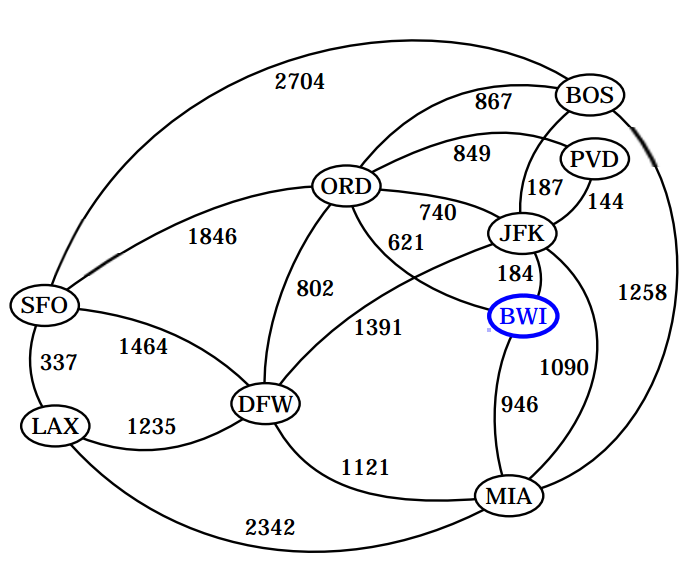
\includegraphics[scale=0.5]{graphe.png}
%     \caption{Graphe}
% \end{figure}

% \section*{Exercice 5}

% Dans certaines applications (les réseaux notamment), une architecture de graphes
% est utilisée et un des noeuds joue souvent un rôle spécial par rapport aux
% autres (e.g., un serveur de fichiers au sein d'un réseau d'ordinateurs). Pour
% obtenir des performances optimales, on souhaiterait déterminer ce noeud comme le
% "centre" du graphe. Pour cela, on définit, étant donné un graphe $G$ et un noeud
% $v$, l'excentricité de $v$ comme la longueur du plus long des plus courts
% chemins entre $v$ et tous les autres noeuds de $G$. Le centre de $G$ est défini
% comme le noeud d'excentricité minimale.

% \begin{enumerate}
% \item Proposer un algorithme pour calculer le centre d'un graphe $G$.
% \item Quelle est sa complexité si $G$ est implémenté par une liste d'adjacences?
% \item  Quelle est sa complexité si $G$ est implémenté par une matrice d'adjacence?
% \end{enumerate}

% \section*{Exercice 6}

% Les échelles de mots sont un jeu (inventé par Lewis Carroll) où l’on doit
% passer d’un mot à un autre en utilisant des mots intermédiaires, et où à chaque étape, une
% seule lettre est enlevée, ajoutée ou remplacée par une autre, les autres restant identiques
% et dans la même position. Toutes les formes grammaticales sont permises. On se restreint
% ici aux mots de même longueur.

% \begin{enumerate}
% \item Passer (en anglais) de LESS à MORE.
% \item Proposer un algorithme pour résoudre ce problème de façon générique, étant donné
% une liste de mots de $n$ lettres.
% \end{enumerate}

\end{document}
